\section{Fundamentação Teórica}
\begin{frame}{Estratégias de Compressão}
    \begin{itemize}
        \item Compressão pós treino: A compressão é realizada apenas após o treinamento do modelo.
        \begin{itemize}
            \item Poda pós treino (Post-training pruning - PTP);
            \item Quantizatição pós treino (Post-Training Quantization - PTQ).
        \end{itemize}
        \item Compressão consciente: A compressão é realizada durante o loop de treinamento.
        \begin{itemize}
            \item Poda consciente (Aware Prune);
            \item Quantização consciente (Aware Quantization);
            \item Poda seguida de quantização (Prune Followed by Quantization).
        \end{itemize}
    \end{itemize}
    Os algoritmos mais convencionais de compressão consciente realizam a compressão apenas uma vez por época, enquanto o algorítmo proposto realiza a compressão a cada mini-batch de cada época do treinamento. 
\end{frame}

\begin{frame}{Compressão consciente por poda}
Uma das abordagens convencionais de compressão das redes neurais é a poda (pruning), que remove parâmetros sistematicamente de um modelo já existente. O desafio é remover uma grande quantidade de parâmetros de forma que afete minimamente a acurácia do modelo.

\end{frame}

\begin{frame}{Compressão consciente por poda}
    \begin{figure}[H]
    \centering
    \includegraphics[width=0.7\textwidth]{figuras/prune_normal_scheme.pdf}
    \caption{Diagrama do loop de aprendizado utilizando poda com controle de época}
    \end{figure}
    As estratégias mais convencionais de poda realizam a remoção apenas uma vez por época. Geralmente no último mini-batch de cada época.
\end{frame}

\begin{frame}{Compressão consciente por poda}
    \begin{figure}[H]
    \centering
    \includegraphics[width=0.7\textwidth]{figuras/prune_scheme.pdf}
    \caption{Diagrama do loop de aprendizado utilizando poda consciente a cada mini-batch}
    \end{figure}
    
\end{frame}

\begin{frame}{Compressão consciente por poda}
A estratégia utilizada para escolher quais pesos devem ser removidos é dada por 
\begin{equation}
    C_k(n) = P(W_k(n),\beta_k) =
    \begin{cases}
      w_k(n) & \text{if } |w_k(n)|\geq \beta_k \\
      0 & \text{if } |w_k(n)| < \beta_k\\
    \end{cases} ,
\end{equation}
onde $\beta_k$ é a janela de corte da $k$-ésima camada definida por
\begin{equation}
    \beta_k = \alpha \times \sigma_k,
\end{equation}
sendo $\sigma_k$ o desvio padrão da $k$-ésima camada e $\alpha$ o valor da agressividade da poda.

\end{frame}





\begin{frame}{Compressão consciente por poda}
    
\begin{figure}[H]
  \centering

  \begin{subfigure}[b]{0.49\textwidth}
    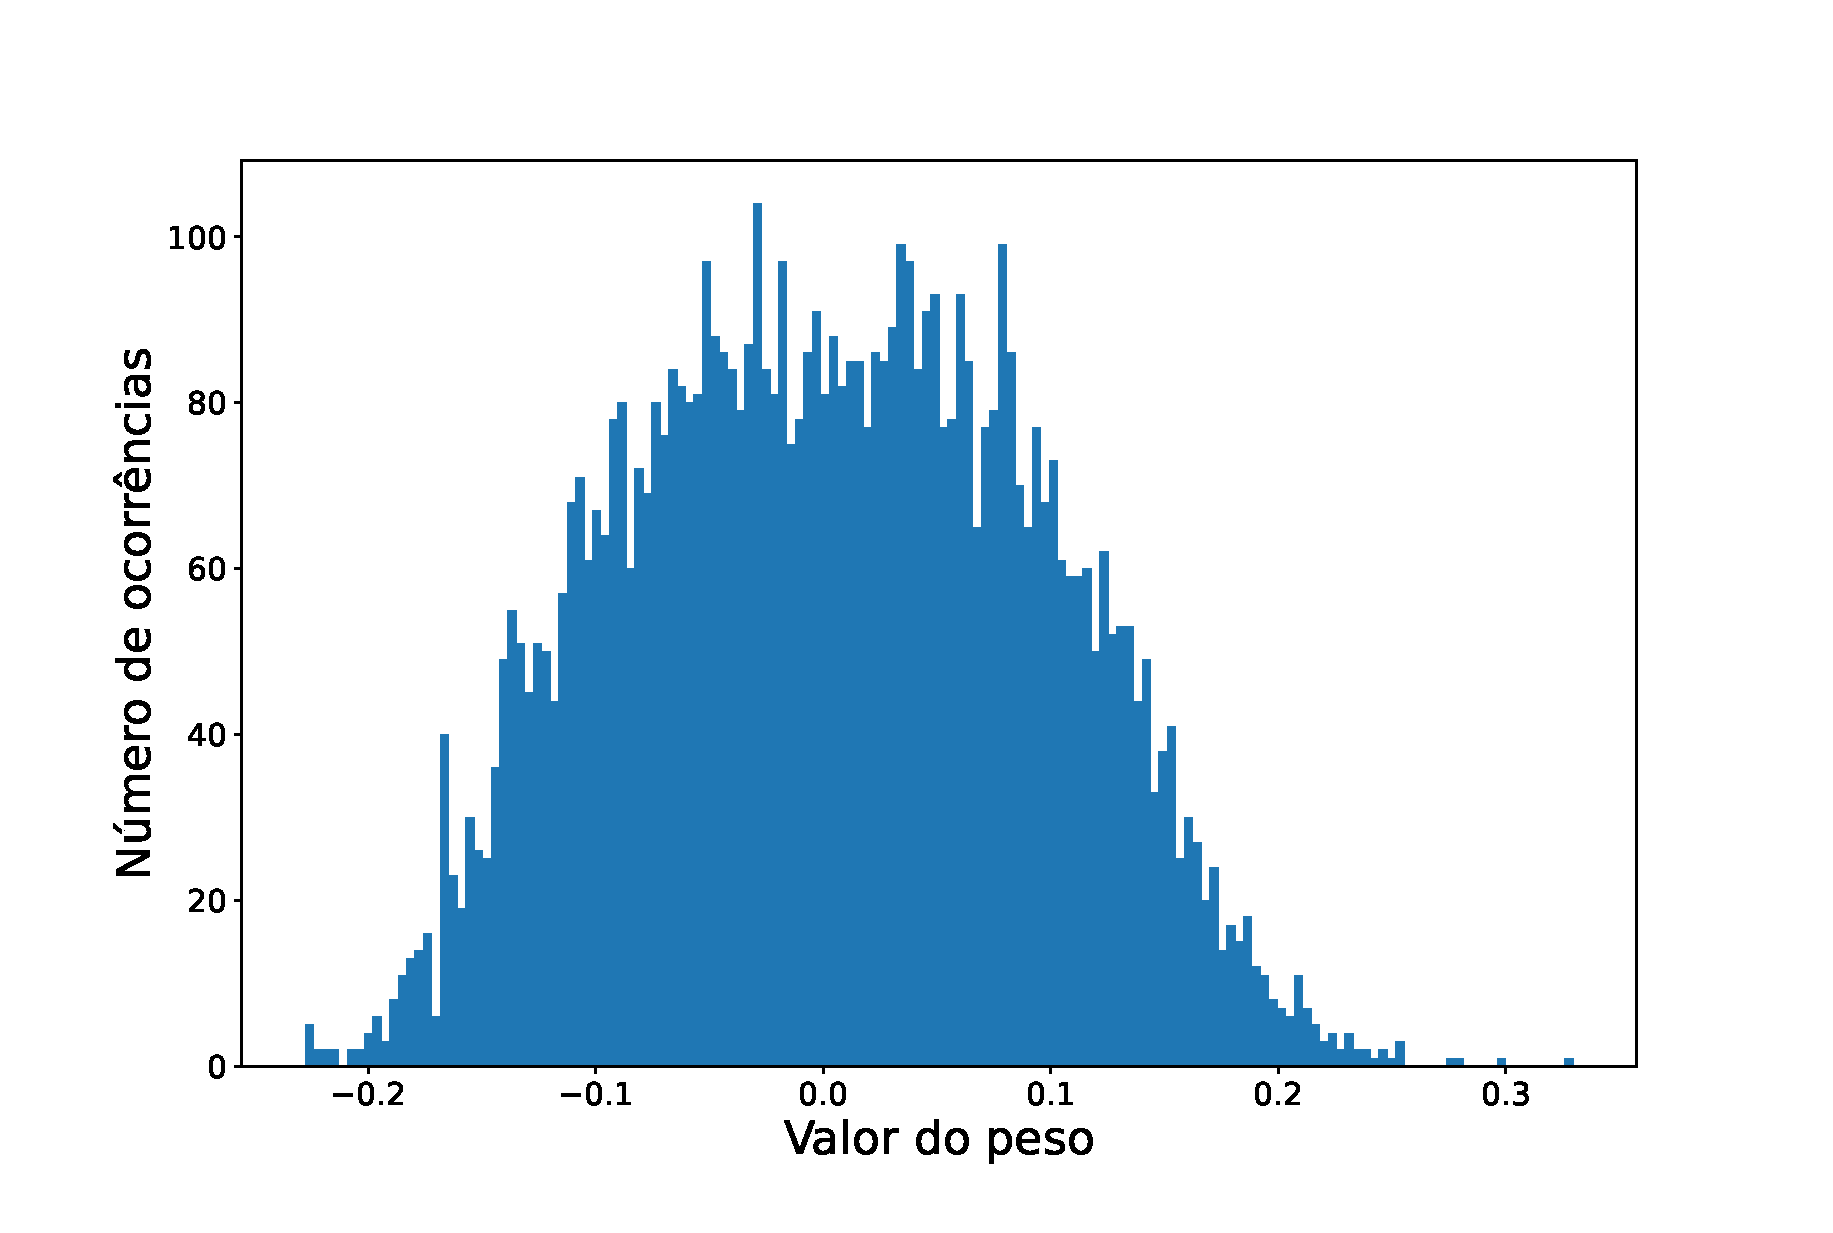
\includegraphics[width=\textwidth]{figuras/hist_weights.eps}
    \caption{Pesos não comprimidos}
    \label{fig:subfig1}
  \end{subfigure}
  \hfill
  \begin{subfigure}[b]{0.49\textwidth}
    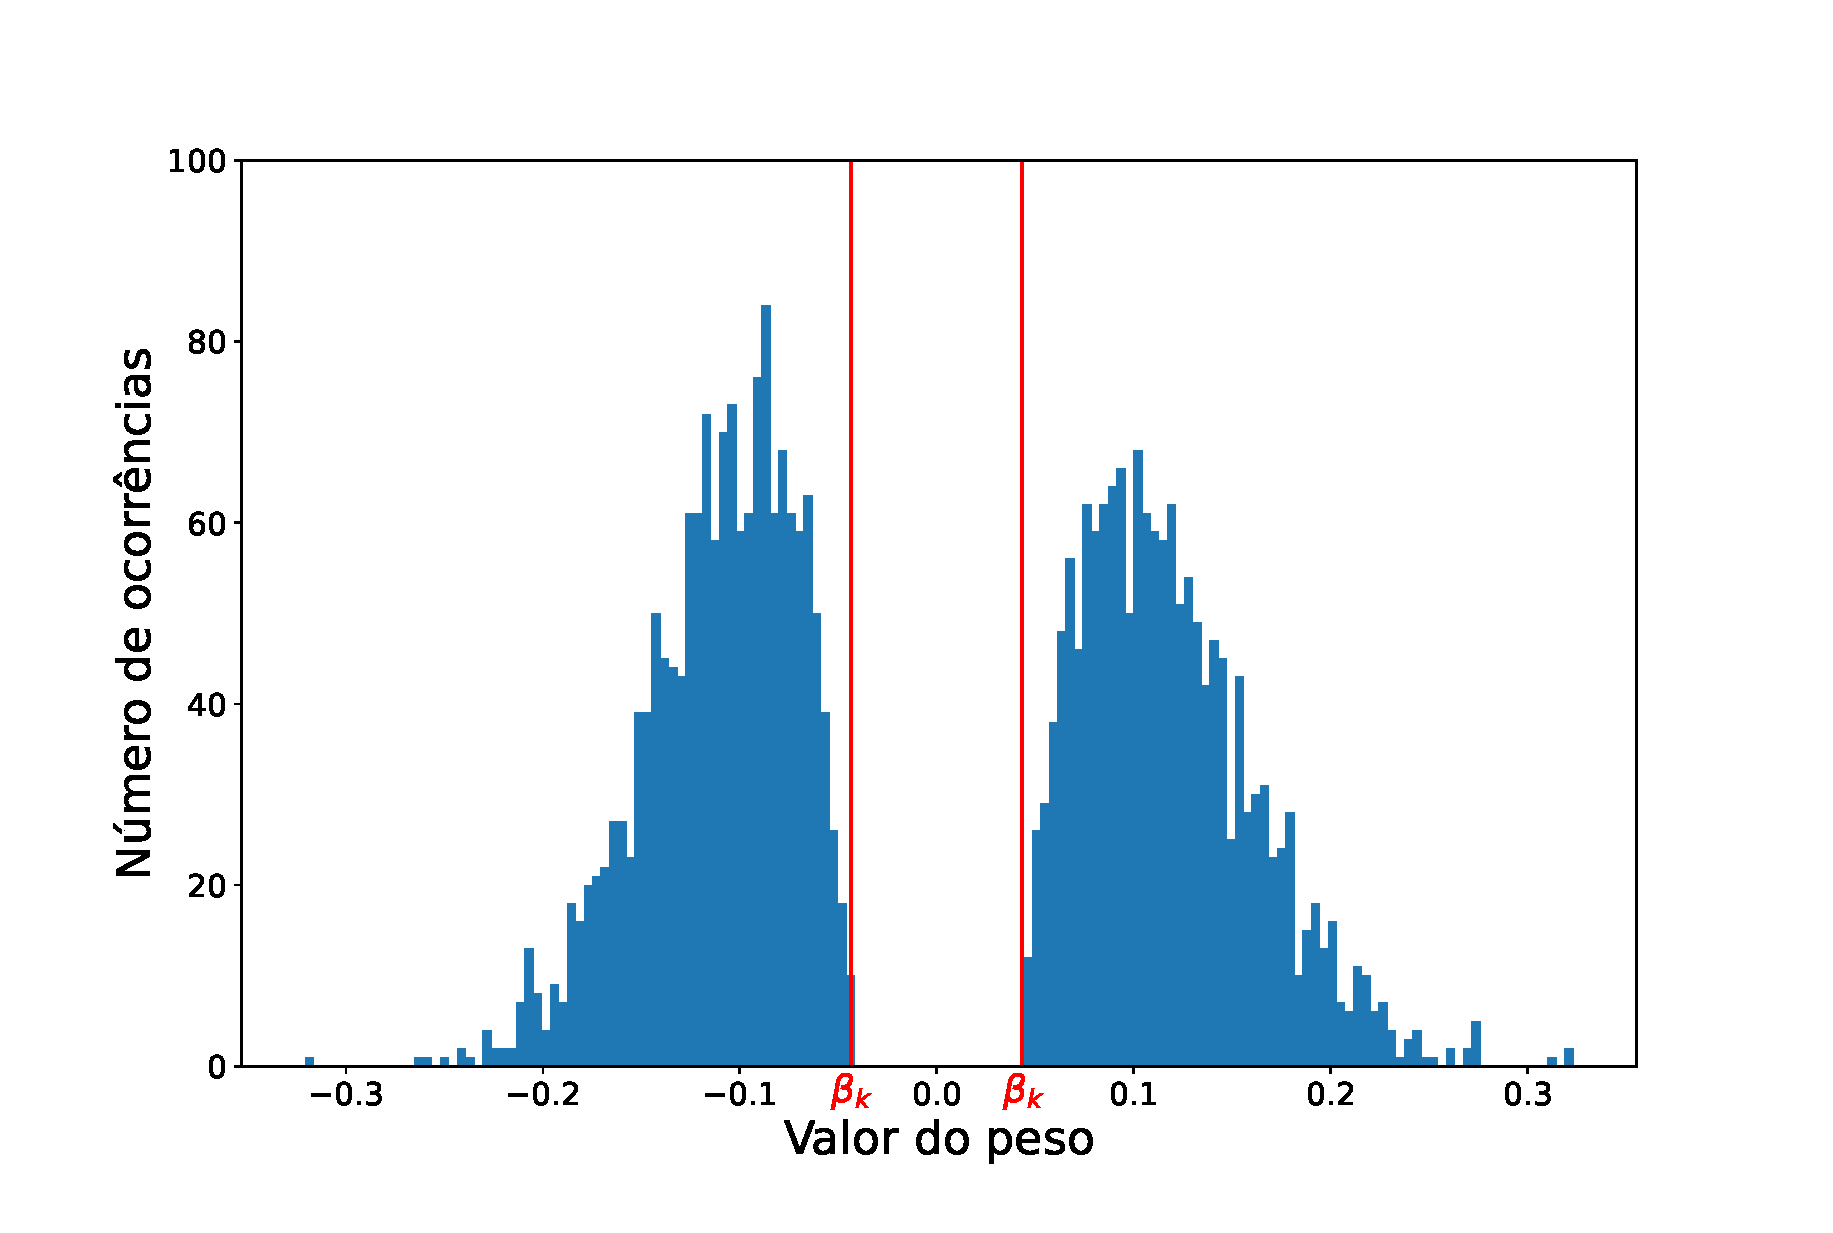
\includegraphics[width=\textwidth]{figuras/hist_prune.eps}
    \caption{Poda consciente}
    \label{fig:subfig2}
  \end{subfigure}

  \caption{Histograma do valores dos pesos associado a um exemplo de compressão de pesos por poda consciente com $\alpha=0,5$  ($\beta_k=0,5 \times \sigma_k$) aplicada à uma camada de uma rede CNN.}
  \label{fig:main}
\end{figure}

\end{frame}

\begin{frame}{Compressão consciente por Quantização}
    A quantização de DNNs é uma estratégia que visa reduzir o consumo de recursos computacionais nas operações matemáticas reduzindo a precisão dos parâmetros da rede diminuindo a representação, em bits, dos seus valores.
    
\end{frame}


\begin{frame}{Compressão consciente por Quantização}
    A estratégia utilizada para quantização de pesos é definida por 
\begin{equation}\label{EqQuantization}
    C_k(n) = Q\left (W_k(n) , q_k\right)= \left \lceil \frac{W_k(n)}{q_k} \right \rfloor \times q_k,
\end{equation}
    sendo $q_k$ definido como o fator de quantização, ou de escala, da $k$-ésima camada 
\begin{equation}
    q_k = \frac{\text{max} \left \{ \left | W_k(n) \right | \right \}}{2^{b-1}-1}.
    \label{ft_quant}
\end{equation}
    onde $b$ é o parâmetro que define a quantidade de bits para quantização.
\end{frame}

\begin{frame}{Compressão consciente por Quantização}
    \begin{figure}[H]
    \centering
    \includegraphics[width=0.7\textwidth]{figuras/quantization_scheme.pdf}
    \caption{Diagrama do loop de aprendizado com quantização}
    \end{figure}
\end{frame}

\begin{frame}{Compressão consciente por Quantização}
    \begin{figure}[H]
  \centering

  \begin{subfigure}[b]{0.49\textwidth}
    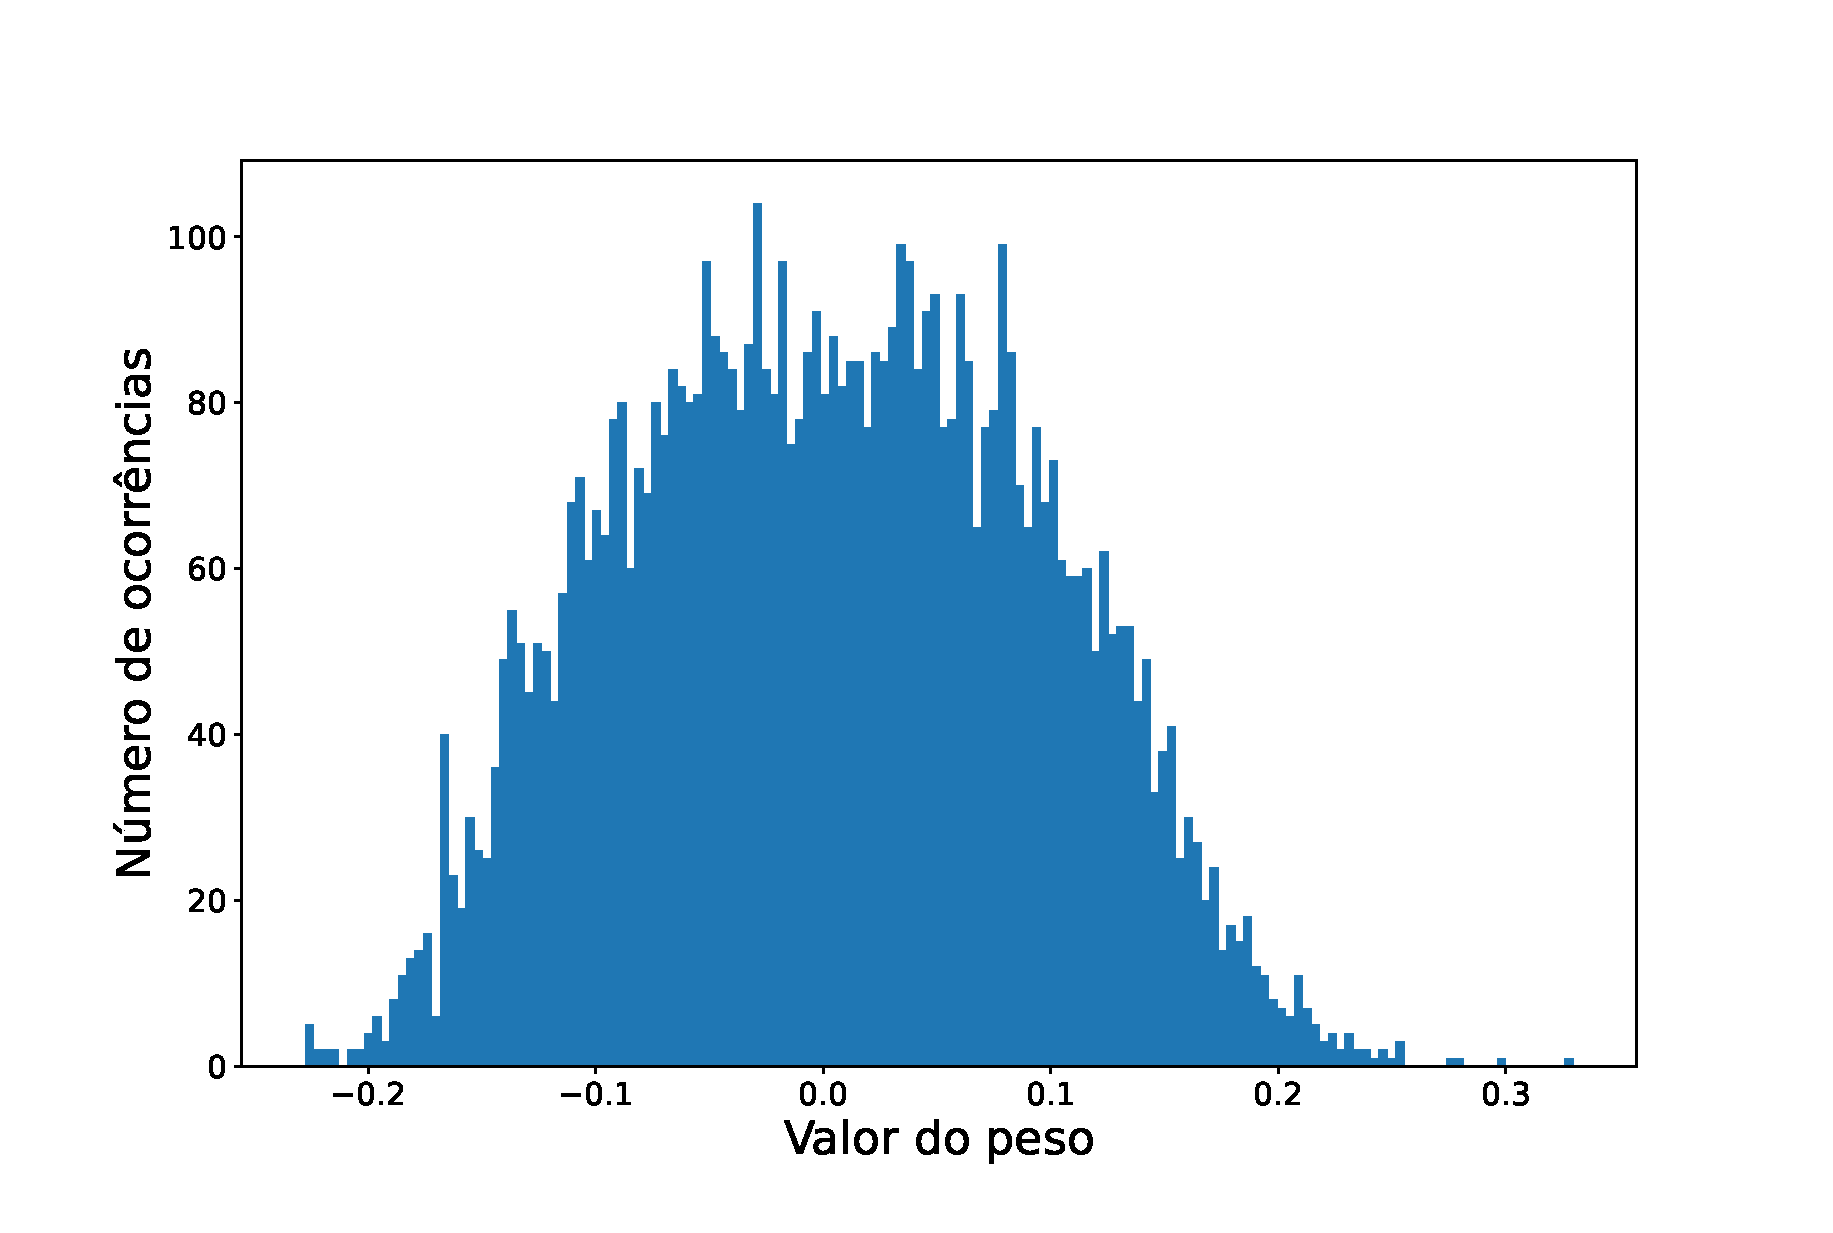
\includegraphics[width=\textwidth]{figuras/hist_weights.eps}
    \caption{Pesos não comprimidos}
    \label{fig:subfig1}
  \end{subfigure}
  \hfill
  \begin{subfigure}[b]{0.49\textwidth}
    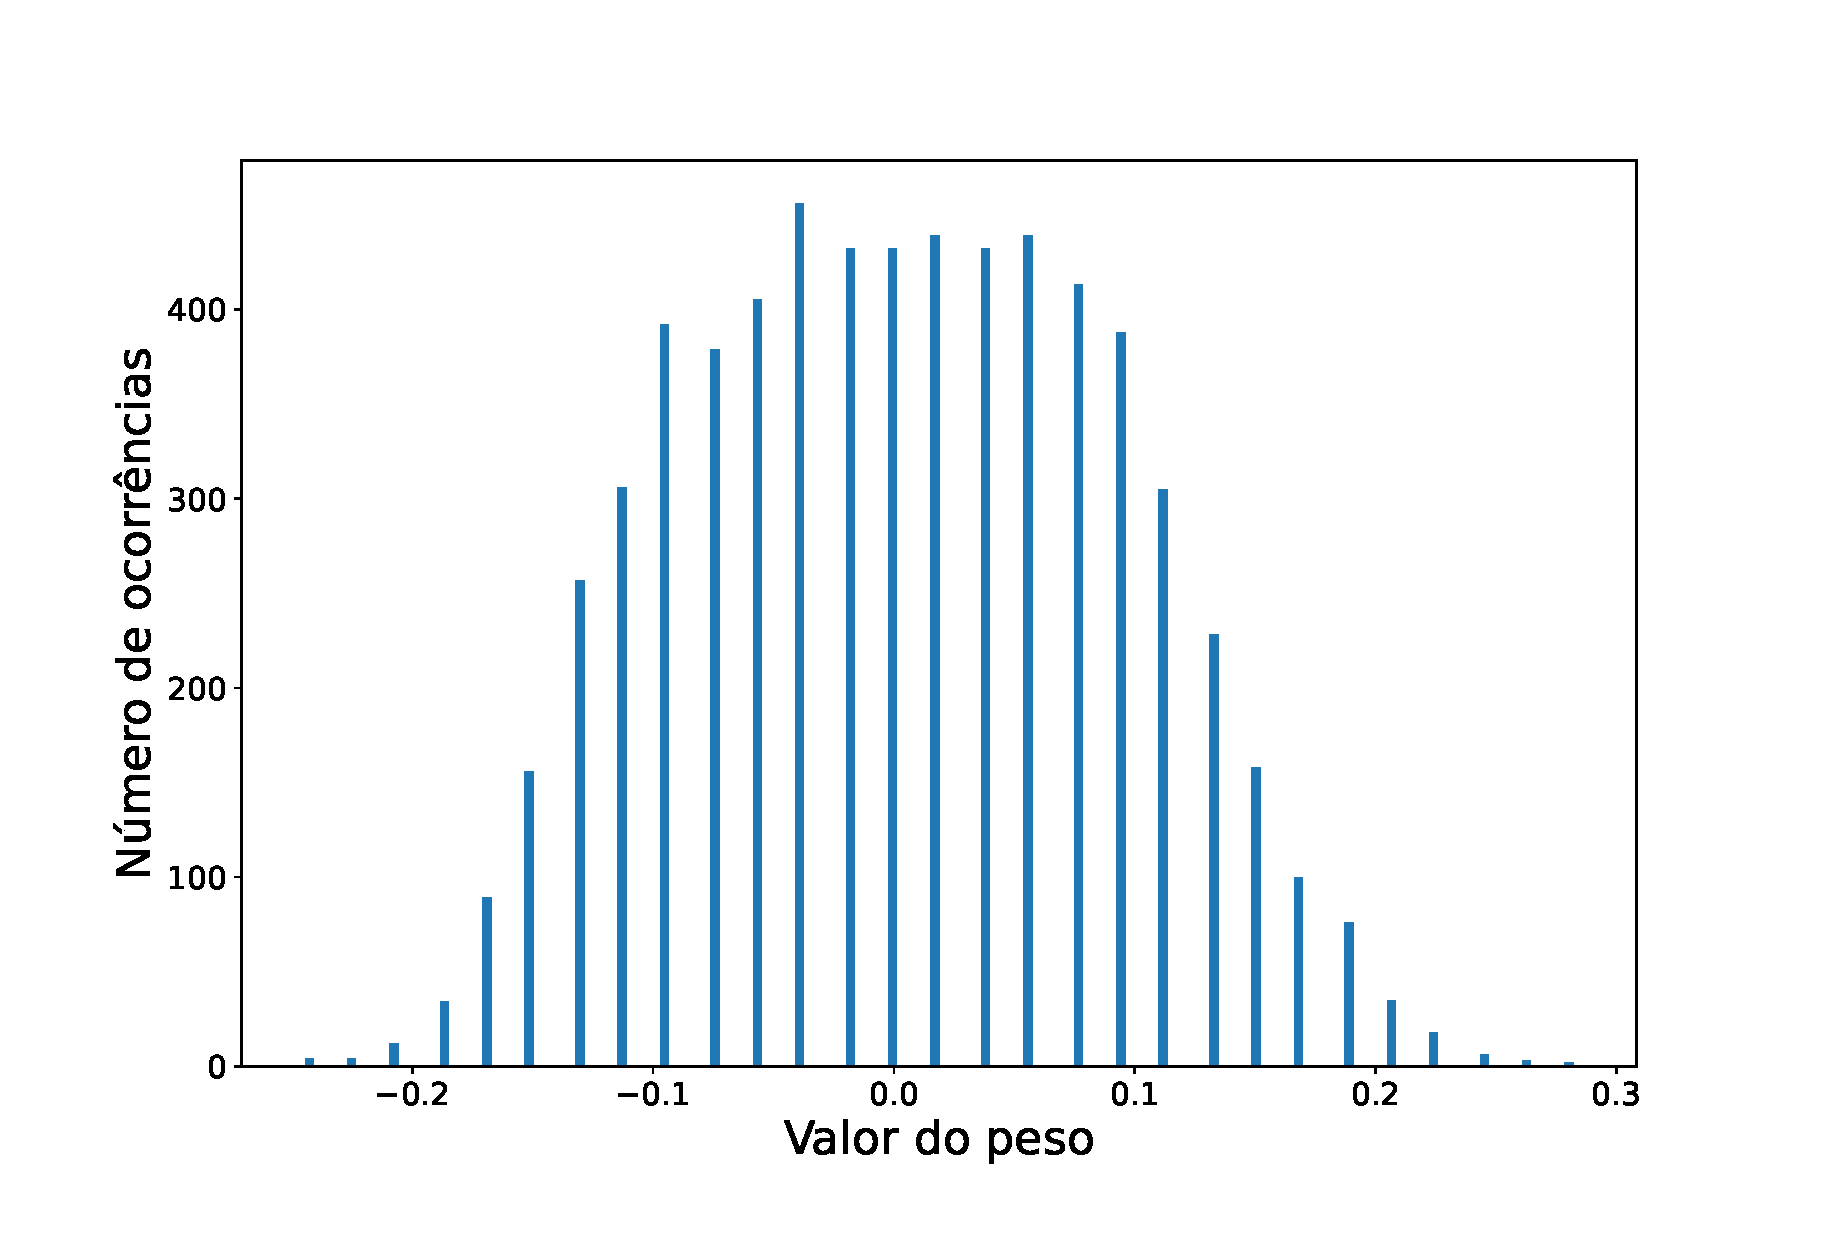
\includegraphics[width=\textwidth]{figuras/hist_quant.eps}
    \caption{Quantização consciente}
    \label{fig:subfig2}
  \end{subfigure}

  \caption{Histograma do valores dos pesos associado a um exemplo de compressão de pesos por quantização consciente com $b=5$ ($M=31$) aplicada à uma camada de uma rede CNN.}
  \label{fig:main}
\end{figure}
\end{frame}

\begin{frame}{Compressão consciente por Poda seguida de Quantização}
    Na compressão por poda seguida quantização, ambas as estratégias são utilizadas durante o treinamento, resultando na remoção de pesos insignificantes e quantização dos pesos remanescentes.
    
\end{frame}


\begin{frame}{Compressão consciente por Poda seguida de Quantização}
    A estratégia utilizada para poda seguida de quantização de pesos é definida por 
    \begin{equation}\label{EqPruningQuantization}
    C_k(n) = Q\left (  P \left ( W_k(n) , \beta_k \right ), q'_k \right),
    \end{equation}
    onde
    \begin{equation}
    q'_k = \frac{\text{max} \left \{ \left | W_k(n) \right | \right \} - \beta_k }{2^{b-1}-1}.
    \end{equation}.

\end{frame}

\begin{frame}{Compressão consciente por Poda seguida de Quantização}
    \begin{figure}[H]
    \centering
    \includegraphics[width=0.7\textwidth]{figuras/prunequant_scheme.pdf}
    \caption{Diagrama do loop de aprendizado com poda seguida de quantização}
    \end{figure}
\end{frame}

\begin{frame}{Compressão consciente por Poda seguida de Quantização}
    \begin{figure}[H]
  \centering

  \begin{subfigure}[b]{0.49\textwidth}
    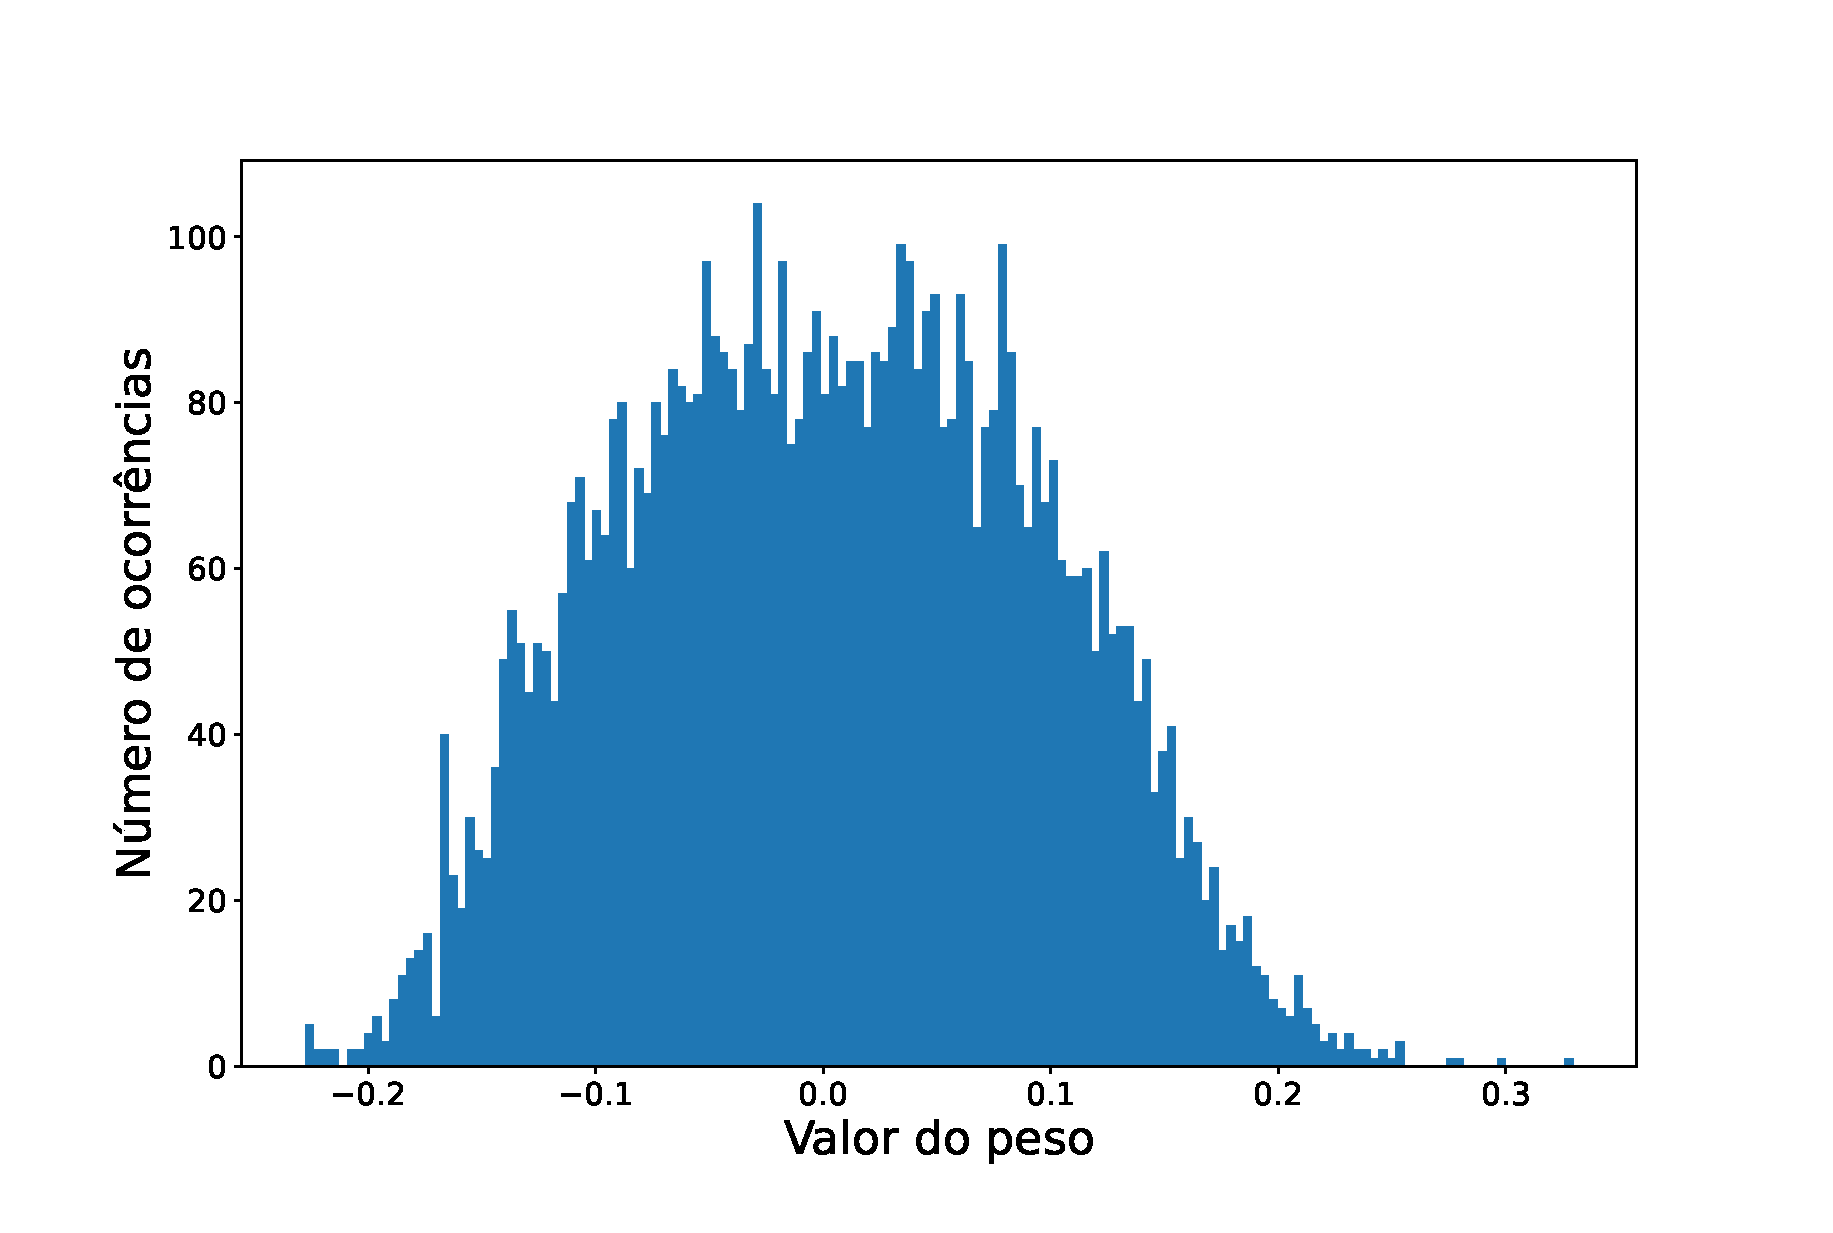
\includegraphics[width=\textwidth]{figuras/hist_weights.eps}
    \caption{Pesos não comprimidos}
    \label{fig:subfig1}
  \end{subfigure}
  \hfill
  \begin{subfigure}[b]{0.49\textwidth}
    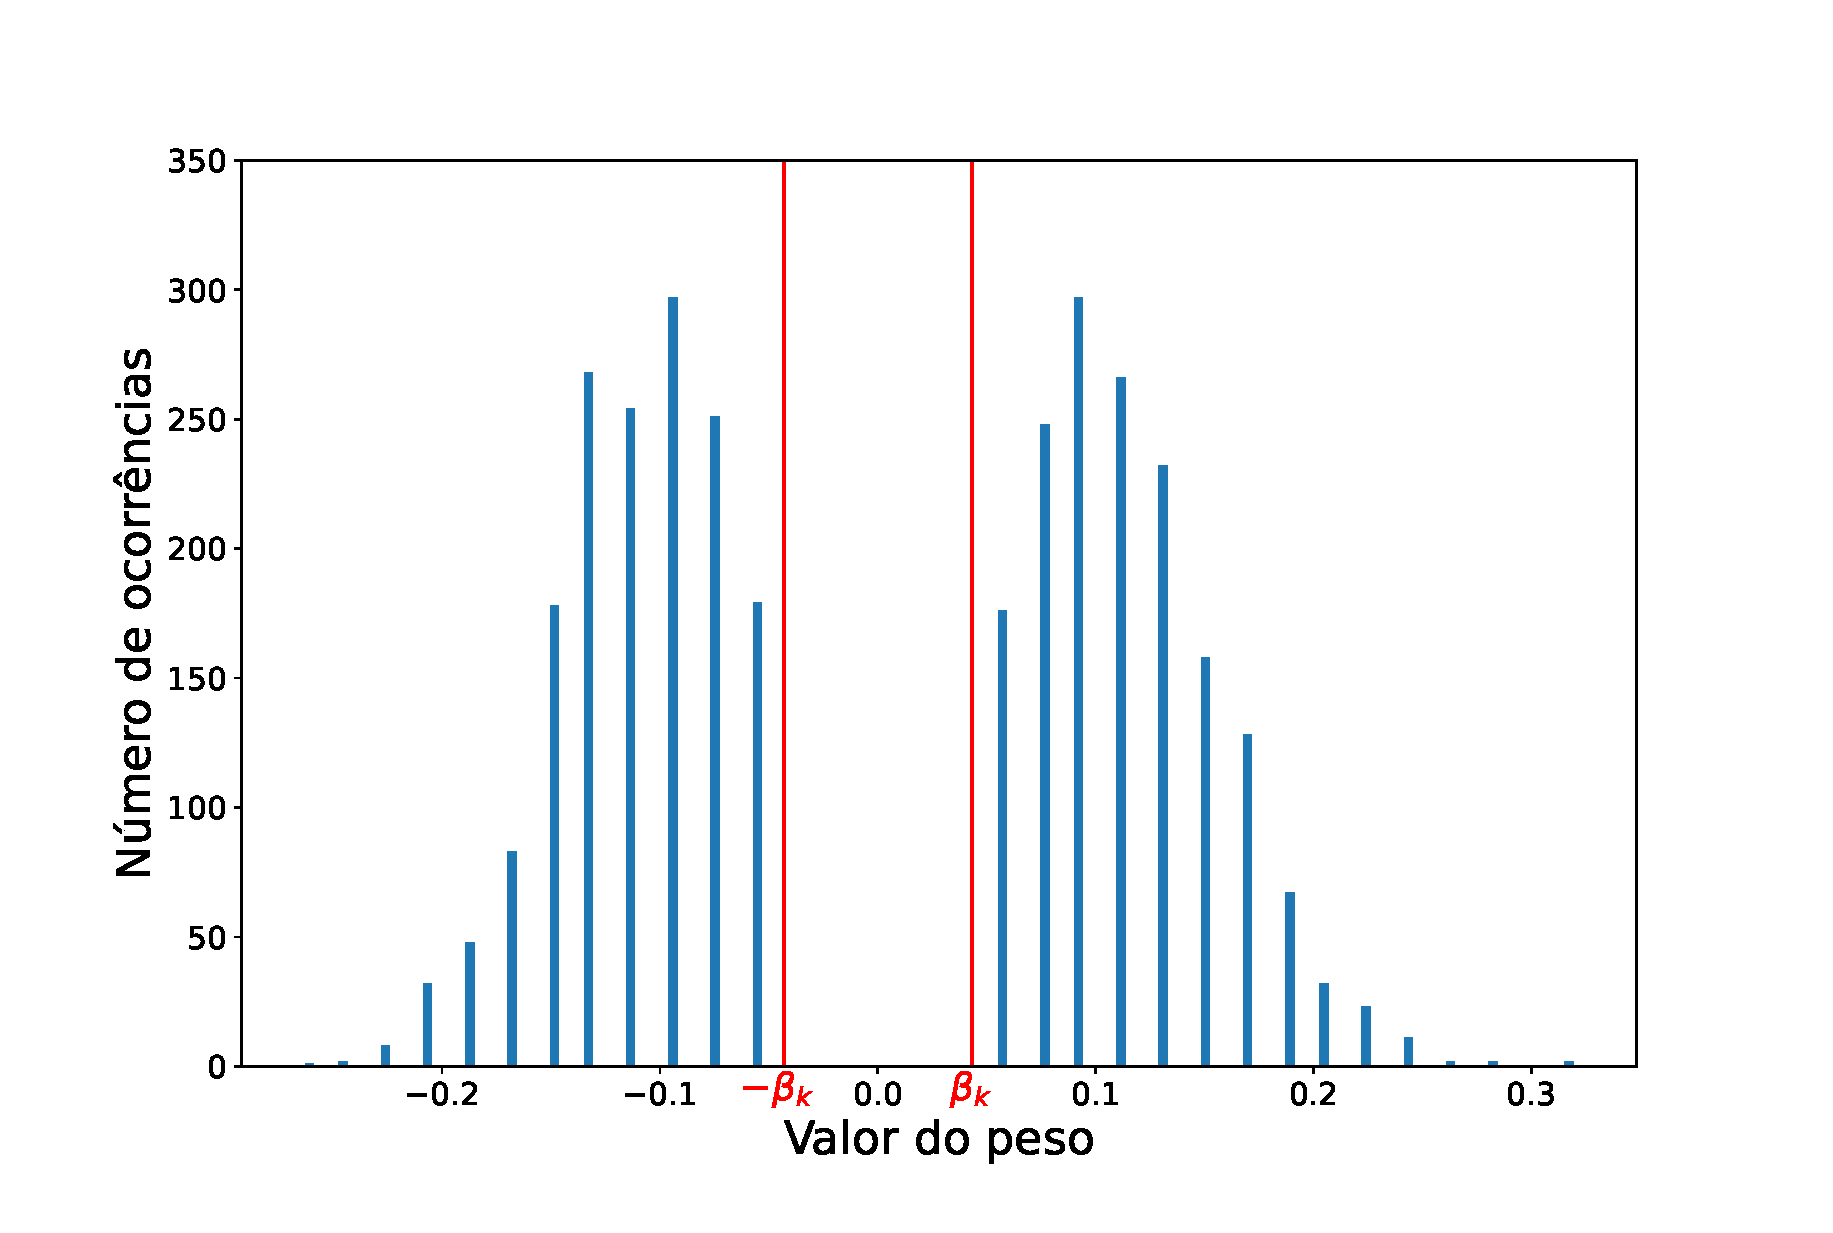
\includegraphics[width=\textwidth]{figuras/hist_prunequant.eps}
    \caption{Poda seguida de Quantização}
    \label{fig:subfig2}
  \end{subfigure}

  \caption{Histograma do valores dos pesos associado a um exemplo de compressão consciente dos pesos por poda seguida de quantização a cada iteração com $\alpha=0,5$ e $5$ bits aplicada à uma camada de uma rede CNN}
  \label{fig:main}
\end{figure}
\end{frame}

\begin{frame}{Geração de modelos comprimidos}
    Após utilização da técnica, o arquivo do modelo gerado precisa ser comprimido. A Para lidar com os modelos que sofreram a compressão por poda, é possível escolher duas estratégias:
    \begin{itemize}
        \item Gerar modelo no formato esparso:
        \begin{itemize}
            \item Modelo gerado salvo no formado esparso CSR ou CSC;
            \item Necessidade de hardwares específicos para operações esparsas;
            \item Modelos com baixa esparsidade podem aumentar o consumo de memória, tempo de inferência e processamento.
        \end{itemize}
        \item Manter formato denso e comprimir a partir de Deflate:
        \begin{itemize}
            \item O arquivo do modelo gerado é comprimido e menor que o original;
            \item Combina as técnicas de Huffman e Lempel-Ziv-Storer-Szymanski para compressão do modelo;
            \item A infererência é feita com o modelo no formato denso (pesos supostamente removidos).
        \end{itemize}
    \end{itemize}
\end{frame}

\begin{frame}
    Para a estratégia de quantização, os parâmetros do modelos são transformados para uma representação em bits, sendo calibrados a partir do fator de quantização $q_k$.
\end{frame}